\chapter{A climatology of urban surface heat islands derived from hemispherical radiometric surface temperatures}

\section{Introduction}

The temperature of the surface is integral in understanding, predicting, and modeling boundary-layer air temperature patterns, surface energy balances, and, in urban areas, has important implications for human thermal comfort and building energy usage. Urban modification of surface geometry and thermal, radiative, moisture, and aerodynamic properties results in differential surface heating and cooling patterns and strong microscale spatiotemporal variations in urban surface temperature (T\textsubscript{surf}). Integrated up to larger scales, urban areas tend to store and generate more heat relative to non-built surroundings which manifests in elevated T\textsubscript{surf} and T\textsubscript{air} a phenomenon termed the urban heat island effect (UHI). To foster a more complete understanding of the effect of urban areas climates across scales, accurate, spatiotemporally continuous and geometrically representative characterization of T\textsubscript{surf} in cities has long been a goal in urban climatology. The proliferation of satellite and aerial thermal infrared (TIR) remote sensing has enabled spatially-extensive characterizations of surface climates at ever improving spatial and spectral resolutions. Such campaigns have elucidated urban T\textsubscript{surf} and surface urban heat island (sUHI) patterns globally at large spatial scales. However, technological improvements in TIR remote sensing have yet to address a three potential sources of error when applied in urban areas: 

\begin{enumerate}
	\item Geometric undersampling of 3-dimensional terrain
	\item Temporal discontinuity in overpass cycles and sensor sampling regimes
	\item Clear-sky bias
\end{enumerate}

\noindent These biases present a potentially significant source of error by failing to capture micro-scale temporal and geometric variations in urban T\textsubscript{surf} and sUHI. 

Inter-site comparison is the crux of UHI analysis, thus it is imperative that urban T\textsubscript{surf} measurements are representative of coherent urban patches and free from confounding influences (i.e. atmospheric and emissivity effects). Meta-analysis of air temperature (T\textsubscript{air}) UHI literature shows that these goals are rarely satisfied \citep{Stewart2011}. Given the relative difficulty in retrieving accurate, representative urban T\textsubscript{surf}, similar conclusions are likely for sUHI analysis. In spite of this fact, and the short period over which large-scale, generalizable methods for measuring urban T\textsubscript{surf} have been available, study of sUHI via TIR remote sensing has expanded significantly in the last twenty years \citep{Peng2012,Voogt2003}. Using the method described in Chapter \ref{paper1} we derive an 8-month climatology of hemispherical radiometric urban T\textsubscript{surf} (T\textsubscript{hem, r}) from time continuous near-ground upwelling TIR as measured from an inverted pyrgeometer. The method was developed to address and overcome biases inherent in traditional methods for urban T\textsubscript{surf} retrieval by providing temporally continuous, geometrically representative\footnote{A hemispherical view is not perfectly geometrically representative of urban surface geometry. This is best illustrated by visualizing an urban area from the perspective of a downward facing ‘fish-eye’ camera. Geometric sampling biases are a result of lens distortions and the sensor cosine response. However, by sampling the surface 3-dimensionally, T\textsubscript{hem, r} is more representative of urban geometry than conventional 2-dimensional views of the surface. The geometric representivity of urban T\textsubscript{hem, r} is discussed in section \ref{Methodological limitations and considerations}.} urban T\textsubscript{surf} under all-sky conditions for sUHI analysis. These measurements are often made as a part of the net radiation determination for urban energy balance studies.

\subsection{Bias in thermal remote sensing}
Geometric biases in remote sensing of the urban surface are a result of its 3-dimensional, convoluted structure. Compared to flat terrain, complex urban surface geometry modifies receipt of incoming solar radiation and traps a portion of reflected solar and outgoing terrestrial radiation. The resulting microscale spatiotemporal contrasts in urban T\textsubscript{surf} create a directional dependence in observed urban T\textsubscript{surf} when measured from conventional narrow-field-of-view (FOV) TIR remote sensing platforms. Thus, remote sensed urban T\textsubscript{surf} varies based on sensor FOV, viewing angle and direction, and sun-surface geometry - this directional dependence of urban surface temperature is termed "effective thermal anisotropy" \citep{Voogt1998a}. Traditional satellite or airborne remote sensing platforms, by viewing the surface in the nadir, sample only a fraction of the complete urban surface and fail to capture this effect - leading to spatiotemporally variant directional biases of up to 10 \si{\kelvin} in observed urban T\textsubscript{surf} \citep{Voogt1995}. In general, geometric undersampling by a remote sensor in the nadir manifests as an overestimation of daytime T\textsubscript{surf} and an underestimation of nighttime T\textsubscript{surf} \citep{Adderley2015}. However, the magnitude and diurnal and seasonal behaviors of this bias are dependent on sensor viewing geometry and unique site characteristics (canyon height-to-width ratio, canyon orientation and materials, vegetation coverage, etc.). Thus, parameterization schemes to account for urban effective anisotropy are difficult to generalize across urban sites, sensor types, and sensor-surface geometries.

In addition to undersampling the urban surface, most thermal remote sensing platforms yield an instantaneous ‘snap-shot’ and cannot characterize time-continuous T\textsubscript{surf} patterns without sacrificing ground resolution. Temporal discontinuities in thermal remote sensing result in myriad of potential sources of bias over a wide range of time scales. Aerial and satellite thermal remote sensing require clear sky conditions (clouds are opaque with respect to thermal infrared radiation). Hence, long term satellite characterizations of sUHI are biased towards conditions that maximize urban-rural contrasts in T\textsubscript{surf}. This results in an overestimation of “all-sky” sUHI. At diurnal scales, satellite overpass cycles rarely coincide with sUHI maximums and are not standard across cities or platforms. Thus, analysis of sUHI patterns and magnitudes across cities and instrument platforms is difficult. At smaller time scales still, time-continuous analysis of urban T\textsubscript{surf} shows significant microscale (second to minute) fluctuations in temperature \citep{Christen2012}. Most thermal remote sensors provide instantaneous T\textsubscript{surf} (rather than temporally averaged) and are potentially contaminated by high-frequency microscale fluctuations in urban T\textsubscript{surf}. This is particularly salient in urban environments, where a large variety of fabric materials can produce significant directional contrasts in thermal admittance - and thus spatial variations in the magnitude of microscale fluctuations depending on the facet material types viewed by the sensor. The effect of this phenomenon on thermal remote sensing has not been extensively studied, however, the magnitude of microscale fluctuations in T\textsubscript{surf} is significant relative to a typical sUHI signal and thus constitutes a potentially large source of bias.

Both geometric and temporal shortcomings limit the representativity of traditional remote sensed evaluations of urban T\textsubscript{surf} and sUHI. The magnitude of these biases has not been extensively studied, particularly from a long term, climatological perspective. This study presents the first time-continuous, climatological analysis of sUHI retrieved from radiometric hemispherical urban T\textsubscript{surf} retrieved via the correction method described in Chapter \ref{paper1}. These measures are used to assess the magnitude of and overcome geometric and temporal biases inherent in urban TIR remote sensing.

\section{Methods}

This section describes the study area and provides a brief overview of the multiple line-of-sight atmospheric correction method used to derive a time-continuous eight month climatology urban T\textsubscript{hem, r} for sUHI analysis. A thorough discussion of the method is included in Chapter \ref{paper1}.

\subsection{A method to retrieve hemispherical radiometric urban T\textsubscript{surf}}

Remote sensing of TIR is subject to atmospheric influence from gaseous and aerosol absorbers between the surface and the sensor. A pyrgeometer's broad waveband and wide FOV increase the potential for significant atmospheric influence on an observed TIR signal. These effects can result in differences of up to 8 \si{\kelvin} between the 'true' radiometric T\textsubscript{surf} and brightness T\textsubscript{surf} derived from remote sensed observations of upwelling TIR. Atmospheric effects are particularly important when comparing irradiances or remote sensed T\textsubscript{surf} across different study sites and times, as differences in surface geometry, instrument height, and ambient conditions can introduce large spatiotemporal contrasts in the magnitude of atmospheric influence. This is particularly salient for near-ground, broadband radiometers, as band by band spectral atmospheric transmittance can change significantly with path length, shown in Figure \ref{spectransheight}. As inter-site comparison is paramount in understanding the urban effect on T\textsubscript{surf} and is the basis of sUHI analysis, accurate atmospheric correction of remote sensed T\textsubscript{surf} is of prime importance. Thus, urban T\textsubscript{hem, r} in this study are derived using a multiple line-of-sight correction routine which accounts for the 3-dimensionality of the urban surface, changing atmospheric conditions, and spectrally non-uniform sensor response. For each time step, the method generates of modeled at-sensor irradiances for a range of potential T\textsubscript{hem, r} using profiles of measured T\textsubscript{air} and humidity. A corrected T\textsubscript{hem, r} for the target time step is then retrieved by matching the measured irradiance value to the closed modeled irradiance - T\textsubscript{hem, r} pairing. The work flow, described in Figure \ref{flow}, is repeated at 30-minute intervals over the eight month study period to retrieve a climatology of urban T\textsubscript{hem, r} for sUHI analysis.

First, surface-to-sensor path length and view factor geometries are calculated with the surface-sensor-sun urban model (SUM) \citep{Soux2004}. Using a digital building model, SUM calculates path lengths from the surface to the sensor and angular view factors by projecting the pyrgeometer FOV onto a simplified (orthogonal) representation of the surface, determining which points in the DBM are 'seen' by the sensor, and calculating the distance from each 'seen' point to the sensor. Path lengths are binned at 5\si{\degree} intervals and averaged over the azimuth angle. Finally, view factors are calculated for each 5\si{\degree} angular as each bin's proportion of the total view factor and normalized to unity.

Second, version 4.1 of the MODTRAN radiative transfer code \citep{Berk1987} is used to model spectral at-sensor radiances for each angular path length. Runs are initialized using profiles of T\textsubscript{air} and water vapor content collected concurrently at each time step. Spectral radiances are modeled over a bandpass of 1 to 2500 \si{cm^{-1}} at an emissivity of 0.95 and convolved by an extended dome transmittance function to ensure that modeled radiances replicate the actual remote sensed signal. Consultation with radiometer manufacturers made clear the need to extend the modeled bandpass beyond a typical longwave bandpass (approximately 250 - 2500 \si{cm^{-1}}), as silicone domed pyrgeometers are transmissive of radiation in much shorter wavenumber (longer wavelengths) than 250 \si{cm^{-1}} (40 \si{\micro\meter}).

Third, radiances for each angular path length are integrated over the waveband and multiplied their respective normalized view factors. Weighted and corrected angular radiances are integrated over the hemisphere to yield a modeled at-sensor irradiance as ‘seen’ by the pyrgeometer for the target T\textsubscript{hem, r}. 

For each time step, the above steps are repeated at an interval of 0.5 \si{\kelvin} for a predefined range of potential T\textsubscript{hem, r}, with results aggregated into a lookup table relating modeled irradiances to corrected T\textsubscript{hem, r} for the observed ambient T\textsubscript{air} and humidities. The measured irradiance is then matched with the closest modeled irradiance to return the associated corrected T\textsubscript{hem, r} for the target time step. sUHI magnitudes for the study area are calculated as the difference between urban T\textsubscript{hem, r} and rural T\textsubscript{hem, b} with rural T\textsubscript{hem, b} calculated via

\begin{equation}
\label{ruralt}
T_{hem,~ b} = \sqrt[4]{\frac{\epsilon L_z^\uparrow + (1 - \epsilon)L_{sky}^\downarrow}{\sigma}}
\end{equation}.

\noindent where $L_z^\uparrow$ is at-sensor upwelling longwave radiation, $L_{sky}^\downarrow$ is at-sensor reflected downwelling longwave radiation, and emissivity ($\epsilon$) = 0.98.

Sensitivity tests included in Section \ref{sensitivity} of the companion paper show that screen level irradiances ($ z $ = ~2 \si{\meter}) are not subject to significant effects from the intervening atmosphere and do not require atmospheric correction. Rural irradiances in this study were measured from approximately 2 \si{\meter} above ground, thus rural T\textsubscript{hem, b} is approximately equal to T\textsubscript{hem, r}.

\subsection{Study area}

T\textsubscript{hem, r} are retrieved from radiation and meteorological data collected from December 2001 through July 2002 as a part of the Basel Urban Boundary Layer Experiment (BUBBLE) campaign conducted in Basel, Switzerland \citep{Rotach2005}. Urban data were observed from a tower located near city center at the "Basel Sperrstrasse" site. Rural reference data were observed at the "Lange Erlen" site approximately 6 \si{\kilo \meter} to the north east in the outskirts of the city of Basel. Urban and rural site morphologies and observed variables are described in Table \ref{morphbspr}.

\begin{table}[H]
	\centering
	\caption{A description of morphological and measured variables for urban and rural sites. Modified from \citet{Rotach2005} to include only relevant parameters.}
	\label{morphbspr}
	\begin{tabular*}{\textwidth}{p{3.75cm} p{2.25cm}p{3.5cm}p{2.75cm}p{2.75cm}}
		\toprule 
		Site & Location & Morphological & Meteorological & Radiation \\ 
		& Height & Characteristics\footnote{} & Variables\footnote{} & [No of levels]\footnote{} \\ 	\midrule
		
		Basel Sperrstrasse \newline \textit{Urban} \textit{street canyon} \newline LCZ: 2 & 47.57\si{\degree} N \newline 7.60\si{\degree} E \newline 255 \si{\meter} a.s.l. & $z_H$ = 14.6  \si{\meter} \newline $\sigma_H $ = 6.9 \si{\meter} \newline H/W = 0.54 \newline $\lambda_C $ = 0.37\newline $\lambda_S$ = 1.0 \newline $\alpha$ = 11.0\% & T\textsubscript{air} [7] \newline H [7] \newline WV [12] \newline WD [1] \newline P [1] & L\textsubscript{up} [3] \newline L\textsubscript{down} [5] \newline S\textsubscript{up} [2] \newline S\textsubscript{down} [3] \\ 
		& & & & \\
		Lange Erlen \newline \textit{Rural parkland} \newline LCZ: B & 47.59\si{\degree} N \newline 7.65\si{\degree} E \newline 240 \si{\meter} a.s.l. & $\alpha$ = 21.4\%  & T\textsubscript{air} [4] \newline H [4] \newline WV [3] \newline WD [1] &  L\textsubscript{up} [1] \newline L\textsubscript{down} [1] \newline S\textsubscript{up} [1] \newline S\textsubscript{down} [1]  \\ 
		\bottomrule
	\end{tabular*} 
		\raggedright
		\textsuperscript{2} Morphological parameters for the Sperrstrasse site were calculated for a 250 \si{\meter} circular area surrounding the study sites using the method described in \citet{Grimmond1999}. $z_H$: average building height, $\sigma_H $: standard deviation of building height, $\lambda_P $: plan aspect ratio, $\lambda_C $: complete aspect ratio, H/W: local canyon height to width ratio, $\alpha$: surface albedo. \\
		\textsuperscript{3} H: humidity, WV: wind velocity, WD: wind direction, P: pressure. \\
		\textsuperscript{4} L\textsubscript{up}: upwelling longwave radiation, L\textsubscript{down}: downwelling longwave radiation, S\textsubscript{up}: upwelling shortwave radiation, S\textsubscript{down}: downwelling shortwave radiation.
\end{table}

During an intensive observation period (IOP) in late June/early July 2002, the Sperrstrasse canyon was instrumented with an array of infrared thermometers (IRT) to view individual canyon facet T\textsubscript{surf} to sample representative road, roof, and wall surface temperatures (T\textsubscript{road}, T\textsubscript{roof}, and T\textsubscript{wall} respectively). Plan and complete aspect ratios for the Sperrstrasse canyon are used to compute weighting schemes to retrieve complete and plan surface temperatures (T\textsubscript{comp} and T\textsubscript{plan} respectively) at 30 minute intervals over the IOP. T\textsubscript{comp} represents an area weighted average complete urban T\textsubscript{surf}, while T\textsubscript{plan} represents the Sperrstrasse site as viewed by a satellite or aerial remote sensor in the nadir. Weighting schemes for T\textsubscript{plan} and T\textsubscript{comp} are included in Table \ref{weightings}. Urban T\textsubscript{surf} derived from complete, plan, and hemispherical representations of the Sperrstrasse site are used to investigate the effect of sensor-surface geometry on remote sensed T\textsubscript{surf} and sUHI, and to quantify the magnitude of geometric biases time-continuously over a range of synoptic conditions. For comparison of sUHI to air temperature UHI, canopy layer air temperature UHI (clUHI) magnitudes are calculated as the difference between urban and rural T\textsubscript{air} measured from 2 \si{\meter} above ground level.

\section{Results}

\subsection{Seasonality in sUHI magnitudes}

Figure \ref{heatsuhi} shows seasonal variations in diurnal patterns of mean monthly hemispherical sUHI magnitudes at 30 minute intervals for the eight month study period. sUHI displays significant seasonal variation, particularly by day, and is strongly controlled by day length and solar angle. Nighttime sUHI does not vary significantly across seasons. 

Figure \ref{heatcluhi} shows seasonal variations in diurnal patterns of mean monthly clUHI calculated at 30 minute intervals for the eight month study period. clUHI development is strongly controlled by the timing of sunset/sunrise cycles and displays the largest seasonal variance in the hours immediately after sunset. Daytime clUHI does not vary significantly across seasons. 
\begin{figure}[H]
	\centering
	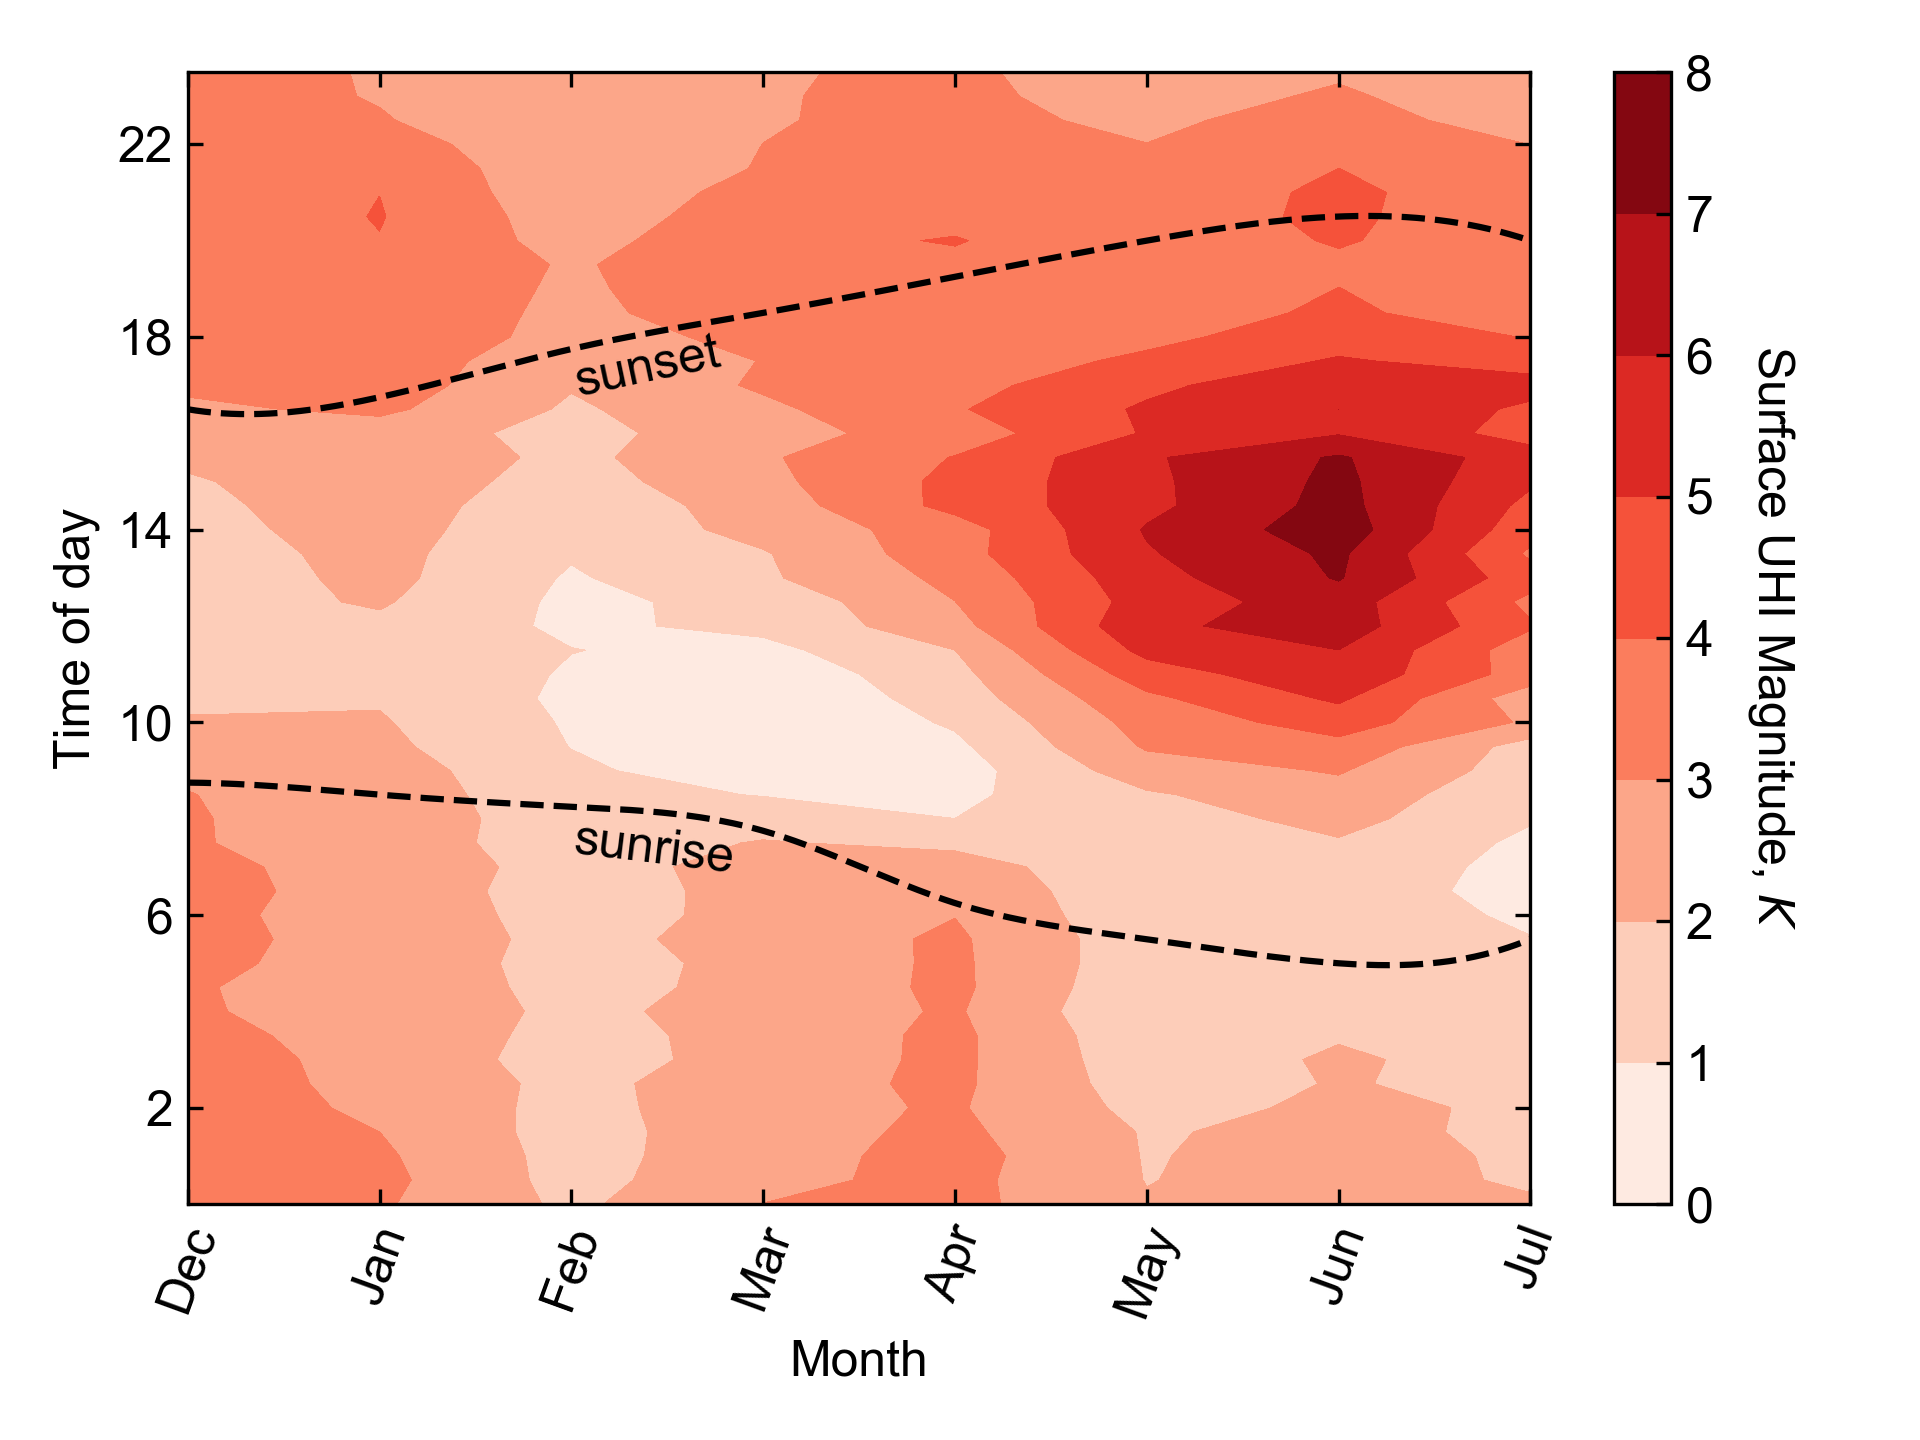
\includegraphics[width=15cm,height=7in,keepaspectratio]{heatsuhi}
	\caption{A heatmap of mean half hourly hemispherical sUHI for each month calculated at 30-minute intervals over the eight month study period.}
	\label{heatsuhi}
\end{figure}

\begin{figure}[H]
	\centering
	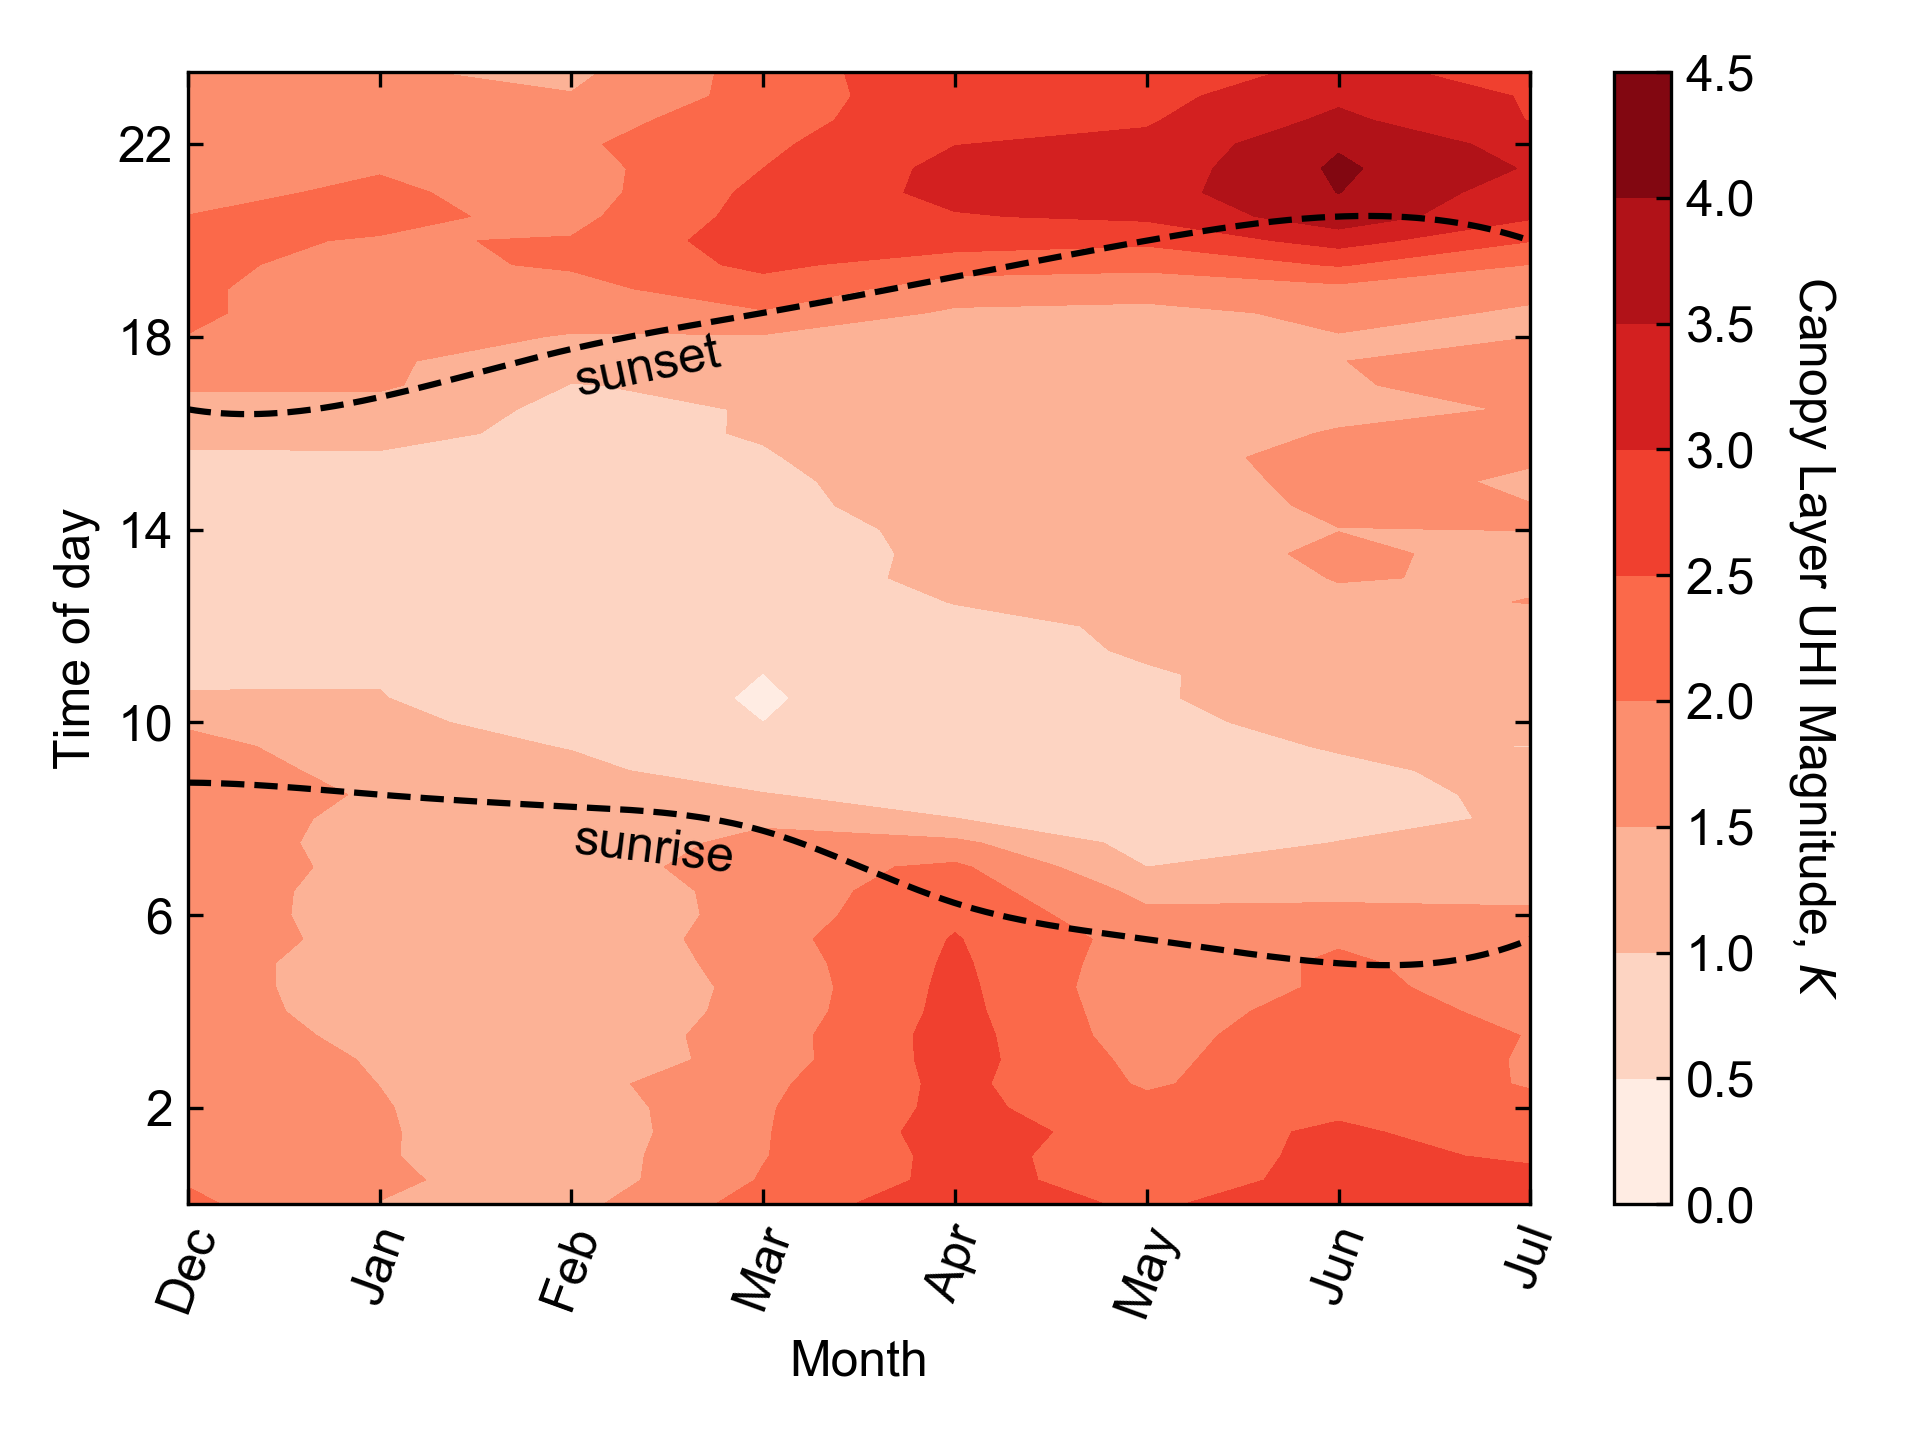
\includegraphics[width=15cm,height=7in,keepaspectratio]{heatatuhi}
	\caption{A heatmap of mean half hourly canopy layer UHI for each month calculated at 30-minute intervals from T\textsubscript{air} measured at approximately 2 \si{\meter} above ground level over the eight month study period.}
	\label{heatcluhi}
\end{figure}

\subsection{The effect of sensor-surface geometry on sUHI}

Figure \ref{bx_suhi_compare} shows sUHI magnitudes calculated from urban T\textsubscript{comp}, T\textsubscript{plan}, and T\textsubscript{hem}. Compared to complete sUHI; nadir and hemispherical views of the surface overestimate sUHI by day and underestimate sUHI by night. sUHI from a nadir view shows the greatest diurnal variance in sUHI, particularly under clear sky 'satellite friendly' conditions. 

\begin{figure}[H]
	\centering
	\includegraphics[width=15cm,height=7in,keepaspectratio]{bxsuhi1}
	\caption{A comparison of sUHI magnitudes from complete, hemispherical, and nadir remote sensed representations of the Sperrstrasse canyon over the IOP. Each plot includes mean sUHI, as well case days representing sUHI under clear sky and clouded sky conditions.}
	\label{bx_suhi_compare}
\end{figure}

\subsection{The effect of meteorological conditions on sUHI}

Figures \ref{meteo_kdown}, \ref{meteo_hum}, \ref{meteo_wv}, and \ref{meteo_atuhi} show sUHI magnitudes as a function of incoming solar radiation, water vapor content, wind velocity, and clUHI. Winter hours are omitted in Figures \ref{meteo_hum}, and \ref{meteo_wv}, and \ref{meteo_atuhi} as sUHI is small and displays minimal variation in winter. Both winter and nighttime hours are omitted in Figure \ref{meteo_kdown} to examine daytime sUHI under clear sky and clouded sky conditions.

\begin{figure}[H]
	\centering
	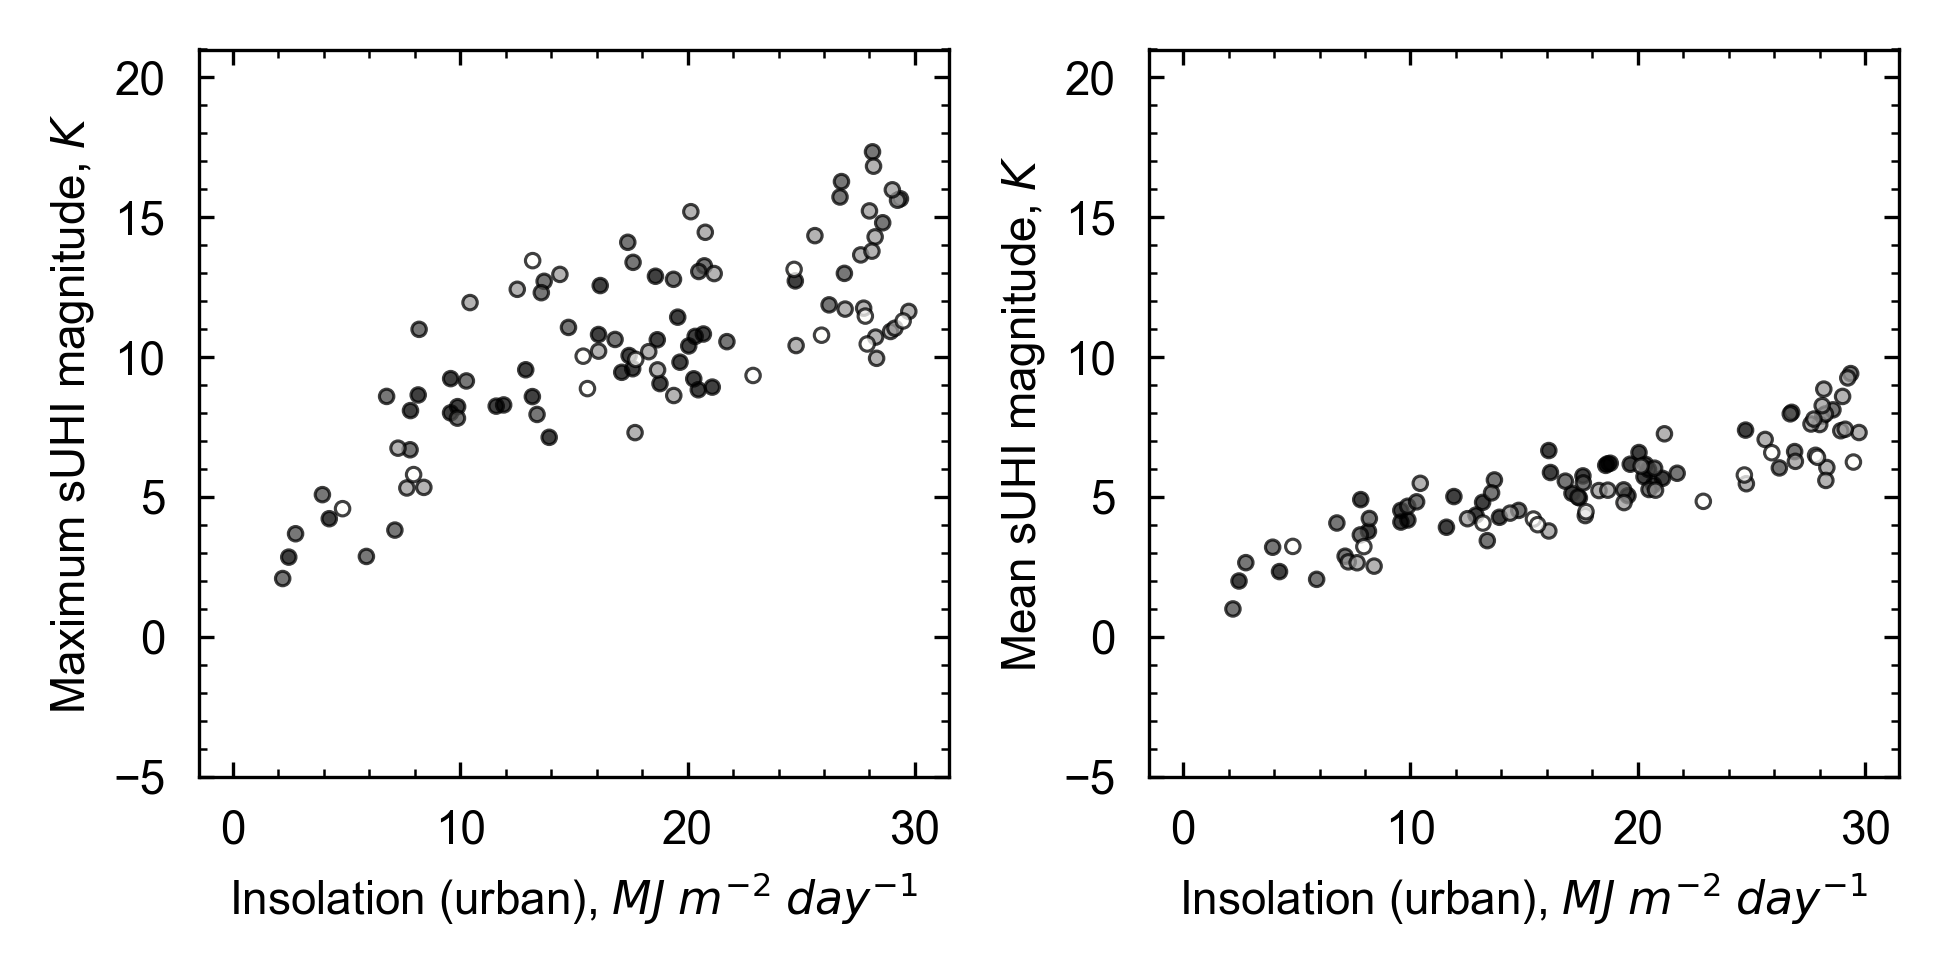
\includegraphics[width=15cm,height=7in,keepaspectratio]{meteo_kdown}
	\caption{sUHI magnitude versus incoming solar radiation binned for clear sky (when the sum of daytime K\textsubscript{down} \textgreater 10000 \si{\watt \per \square \meter}) and cloudy sky days (when the sum of daytime K\textsubscript{down} \textless 10000 \si{\watt \per \square \meter})}
	\label{meteo_kdown}
\end{figure}

\begin{figure}[H]
	\centering
	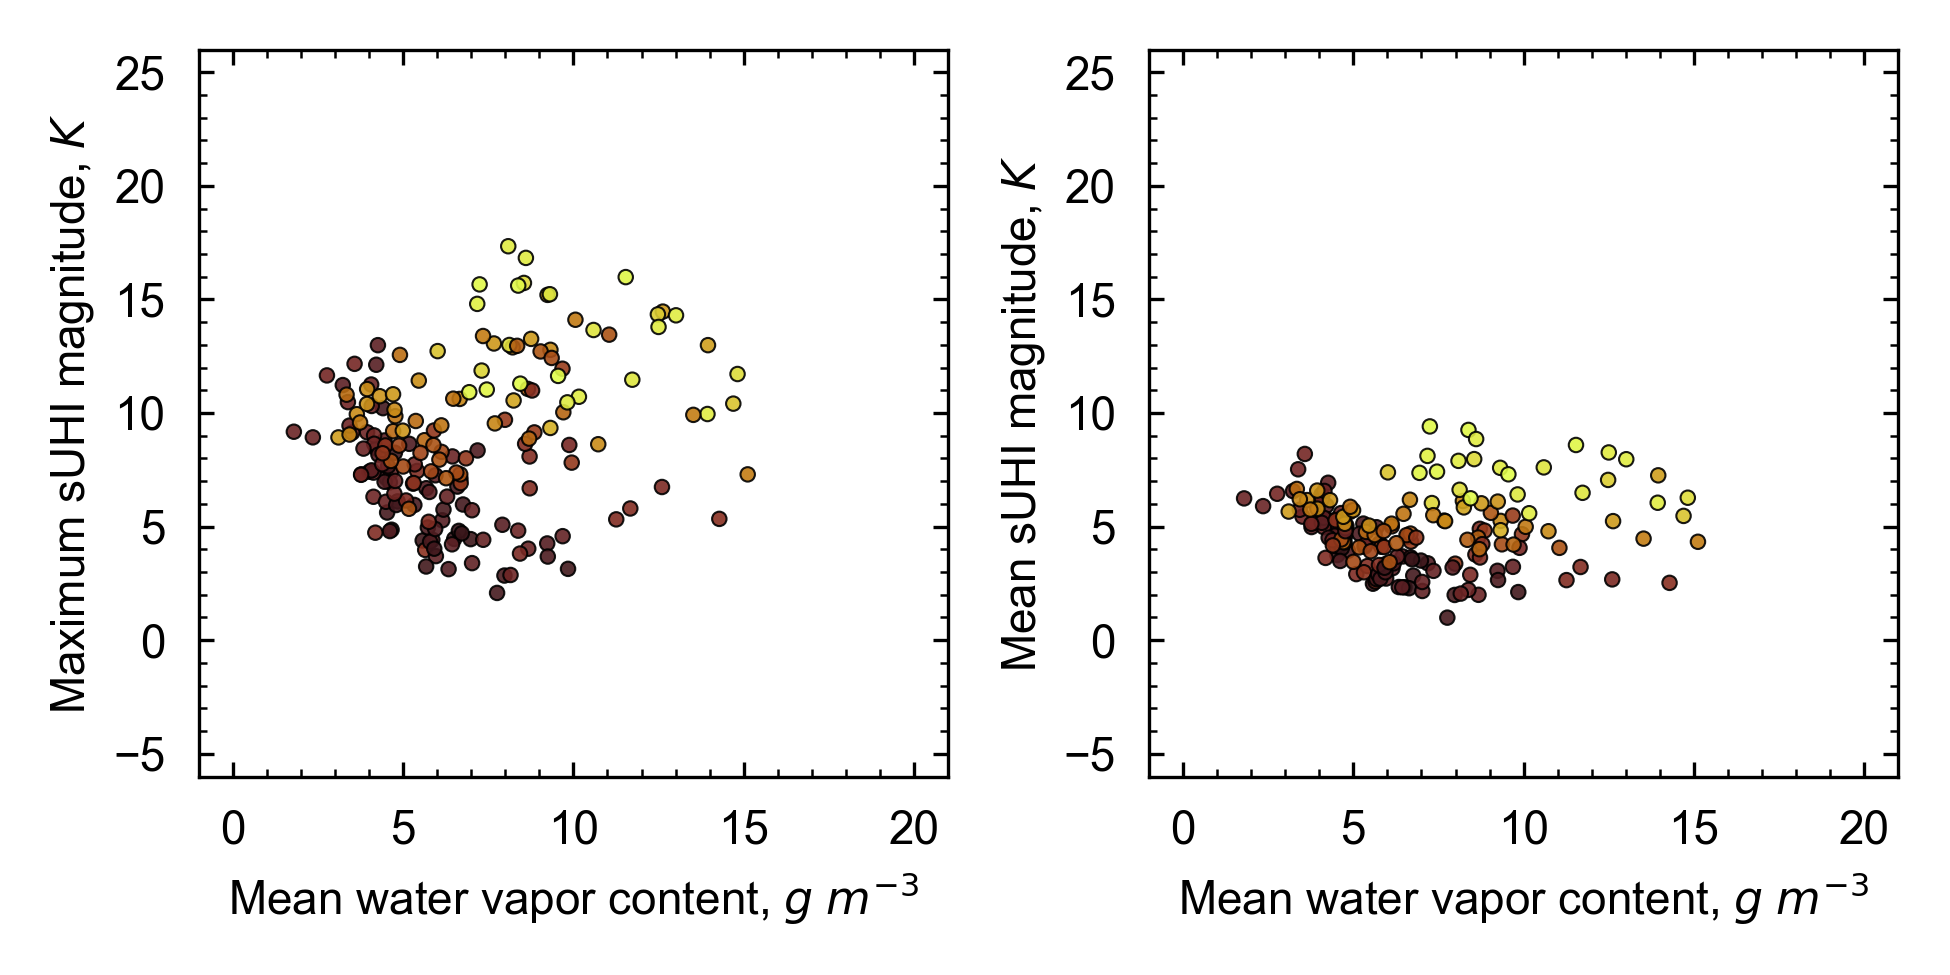
\includegraphics[width=15cm,height=7in,keepaspectratio]{meteo_hum}
	\caption{sUHI magnitude versus atmospheric water vapor content measured at 2 \si{\meter} at the Sperrstrasse site. Similar patterns are observed when rural water vapor content is substituted.}
	\label{meteo_hum}
\end{figure}

\begin{figure}[H]
	\centering
	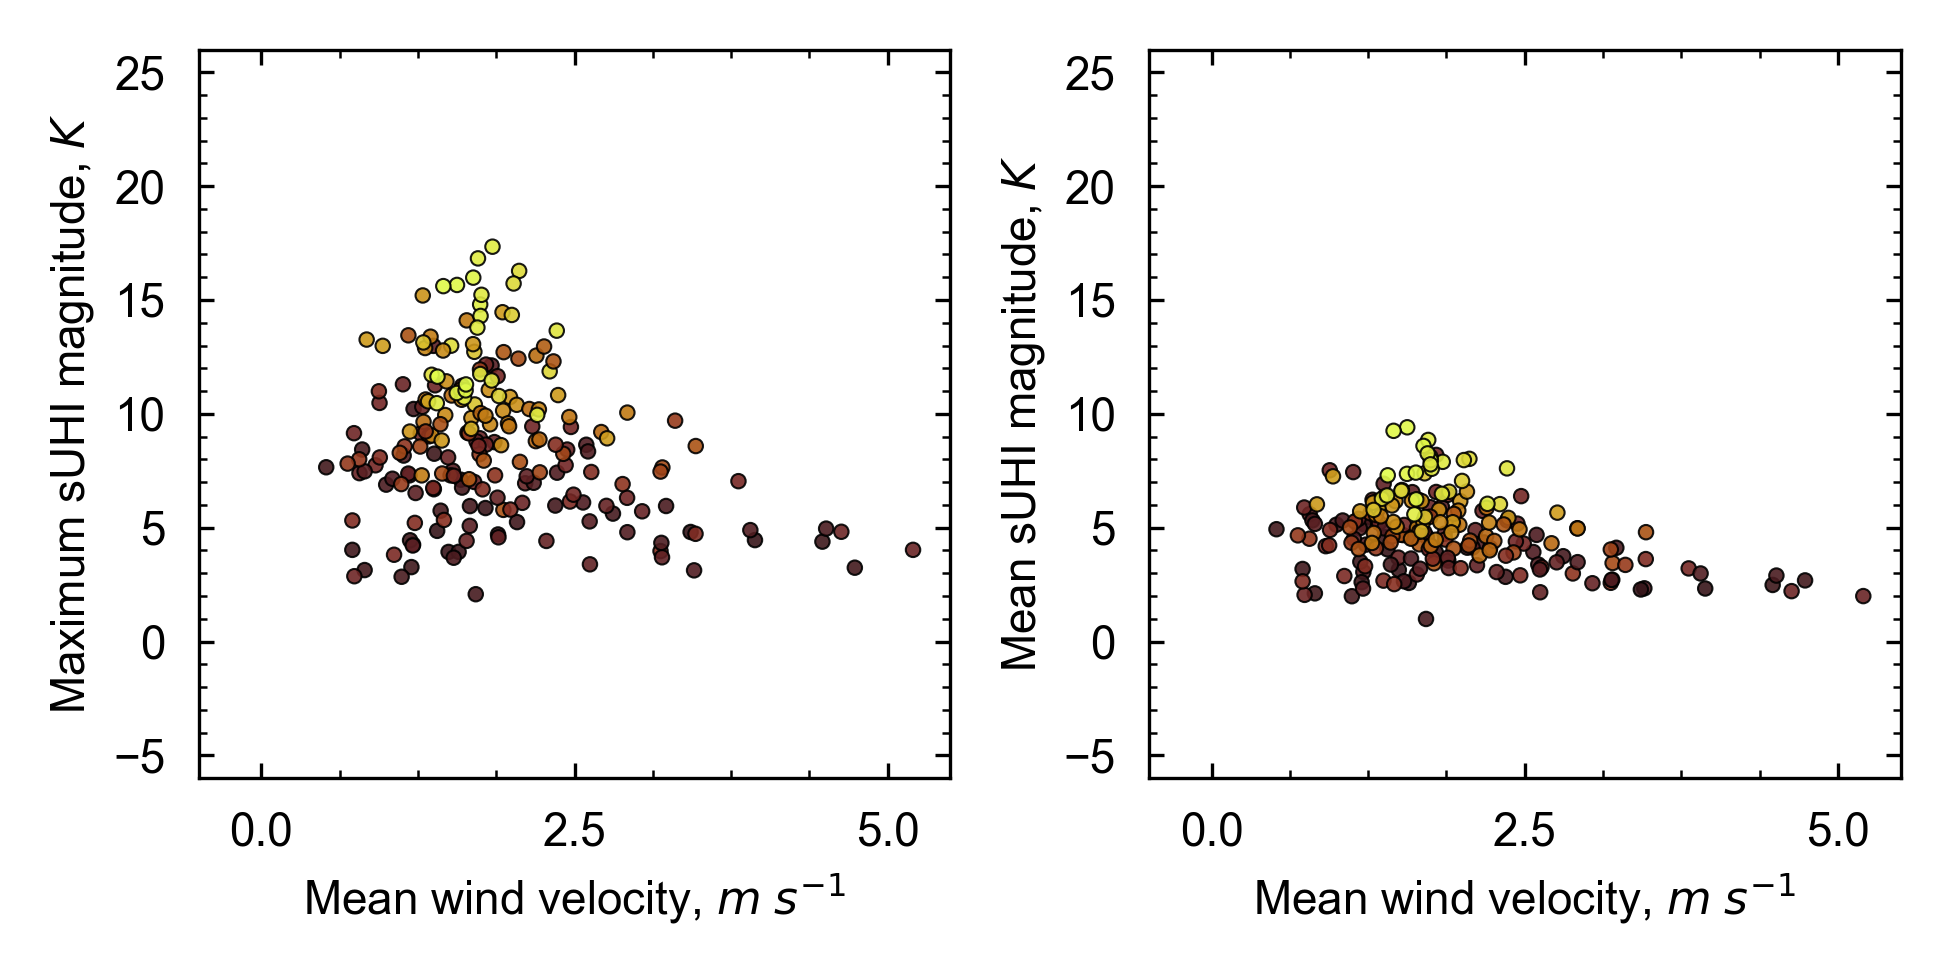
\includegraphics[width=15cm,height=7in,keepaspectratio]{meteo_wv}
	\caption{sUHI magnitude versus rural wind velocity measured at approximately 10 \si{\meter} above ground at the Lange Erlen site.}
	\label{meteo_wv}
\end{figure}

\begin{figure}[H]
	\centering
	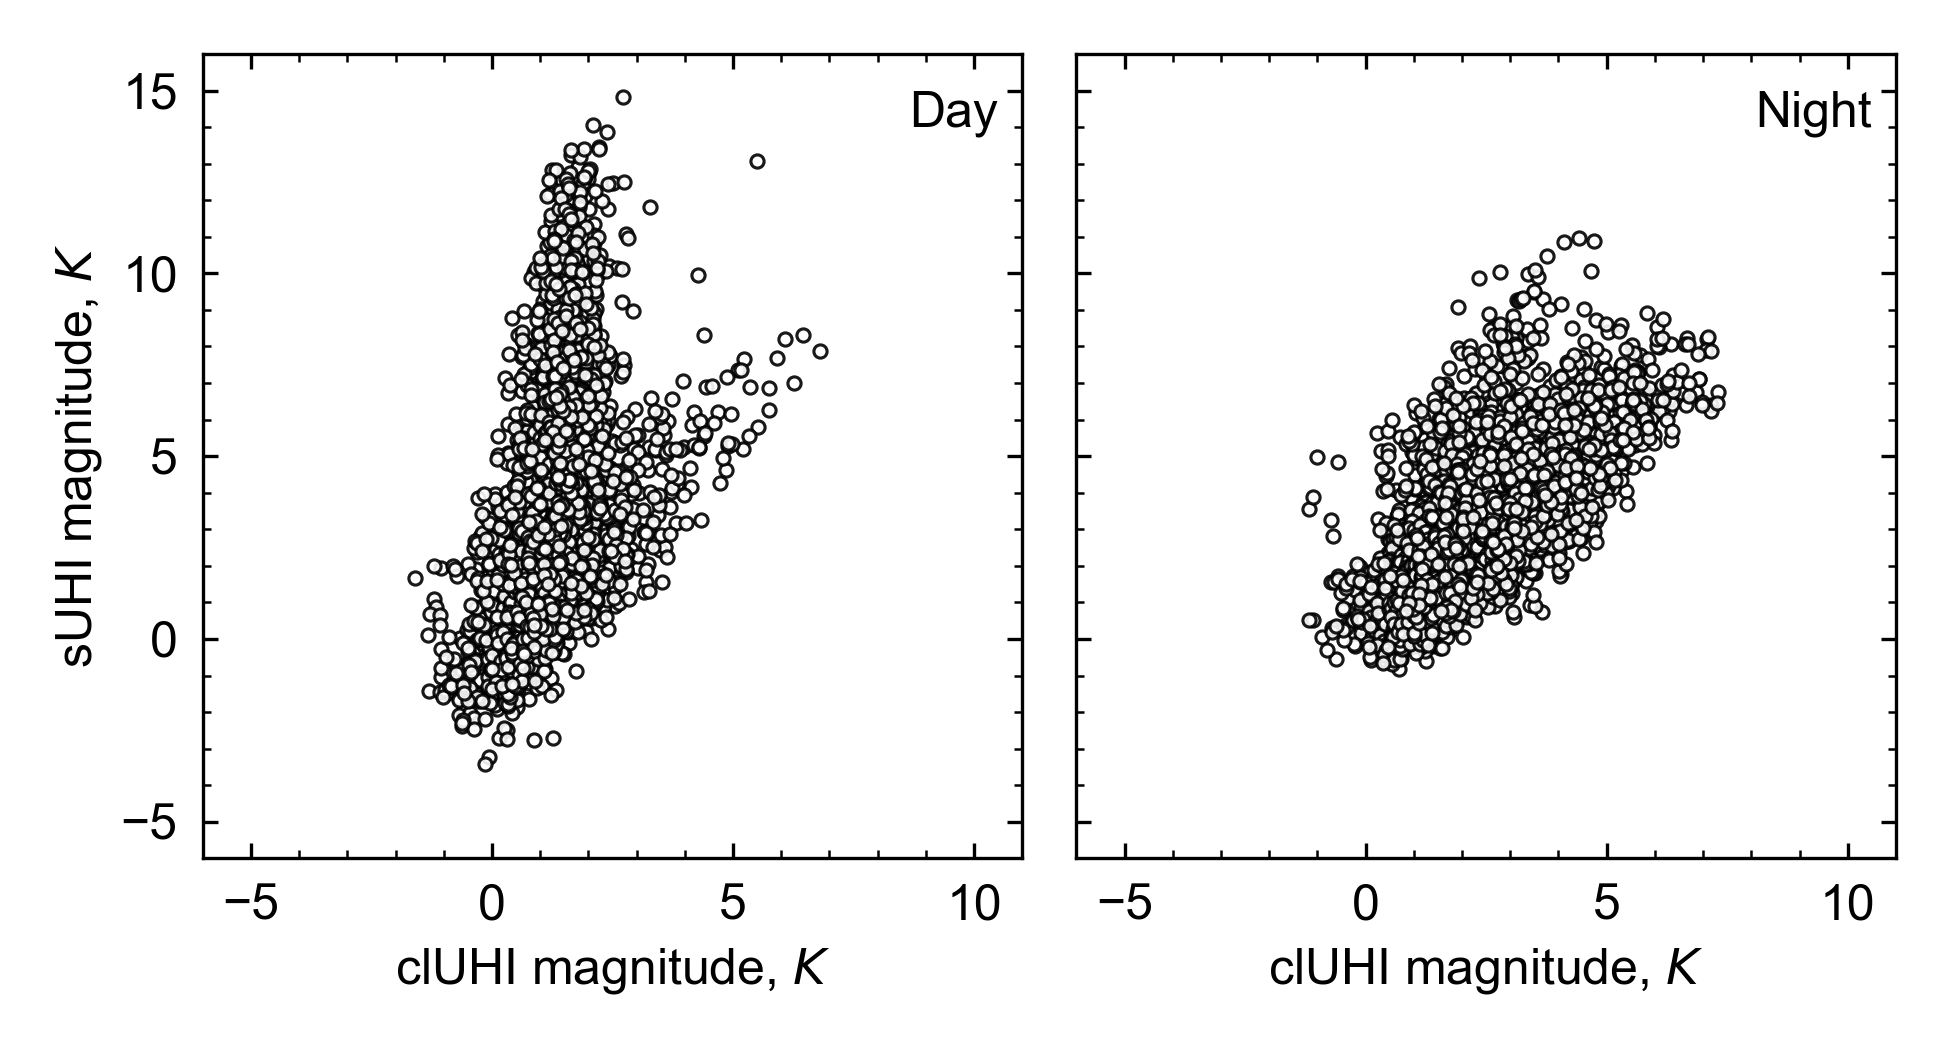
\includegraphics[width=15cm,height=7in,keepaspectratio]{meteo_atuhi}
	\caption{sUHI magnitude versus clUHI magnitude. clUHI is calculated as the difference between urban and rural T\textsubscript{air} measured at 2 \si{\meter} above ground level.}
	\label{meteo_atuhi}
\end{figure}

\section{Discussion}

\subsection{Diurnal patterns of sUHI}

sUHI in Basel from complete, nadir, and hemispherical representations of T\textsubscript{surf} displays two diurnal peaks, the first in the late afternoon and a second just after sunset. Clear sky conditions amplify this phenomena. A late afternoon peak in sUHI is likely the result of the urban-rural contrasts in thermal admittance (and by relation, urban-rural soil moisture contrasts). The thermal admittance of many urban surfaces, particularly rooftops, tends to be lower than rural and vegetated environments \citep{Spronken-Smith1998} – particularly in temperate climates where rural soil moisture is largely maintained through summer. Lower urban thermal admittance manifests in a larger diurnal thermal amplitude and thus, greater daytime surface heating and nighttime surface cooling. Nadir and hemispherical views are biased towards low thermal admittance rooftop facets, and thus display large late afternoon peaks in sUHI.

A second peak in sUHI after sunset is the result of differences in relative cooling rates of urban and rural surfaces. In this case, nighttime sUHI is likely the result of canyon radiation trapping from obstructed canyon sky-view-factors. The second peak sUHI is largest following clear sky conditions when the potential for significant differentials in urban-rural nocturnal cooling rates is maximized. A second peak is observed across all representations of urban T\textsubscript{surf} but is most apparent in complete and nadir representations of sUHI, which, for the Sperrstrasse site, sample T\textsubscript{road} to a greater extent than the hemispherical view. A weak sUHI is maintained through the nighttime as urban and rural cooling rates reach parity in the hours after sunset \citep{Oke2017}. Minimum sUHI is observed just after sunrise, where sUHI magnitudes are occasionally negative. At low solar angles, shading by 3-dimensional urban geometry suppresses heating rates for a large portion of urban surface area, reducing overall urban heating rates in early morning. As solar angles increase through the morning and more facets experience direct isolation, sUHI develops, with nadir and hemispherical representations displaying more rapid intensification than complete sUHI from a bias towards low thermal admittance and directly sunlit rooftop surfaces.

\subsection{Seasonal patterns of sUHI}

Hemispherical sUHI displays significant seasonality, both in terms of its diurnal pattern and overall magnitude. Seasonal variations in sUHI are largest by day, where large seasonal contrasts in cloud cover frequency and solar angle exert strong control on daytime heating rates and sUHI development. Peak sUHI occurs near the summer solstice, when days are longest and isolation on clear sky days is most intense. In winter, daytime sUHI is suppressed from a lower solar input and frequent cloud cover. This weakens wintertime sUHI and shifts its peak to shortly after sunset. Nighttime sUHI is relatively consistent across seasons. Similar seasonality is observed in clUHI, albeit concentrated at different times of day. 

In contrast to sUHI, clUHI is greatest just after sunset and is strongly controlled by sunset/sunrise timing. Peak clUHI occurs just after sunset across seasons, differing only in terms of magnitude, with a larger peak clUHI in summer. However, in this study, it should be note that summertime clUHI magnitudes in the hours just after sunset are slightly higher than expected \citep{Runnalls2000} - possibly the result of cold air draining from hilly terrain west of the rural site. As is the case with sUHI seasonality in clUHI results from seasonal contrasts in solar input and cloud cover frequency. Increased wintertime cloud cover reduces radiative losses by the canyon air volume after sunset, suppressing mean wintertime clUHI magnitudes. Daytime clUHI is consistently small across all seasons. Thus, although sUHI and clUHI are controlled by similar climatic controls and have a similar micro meteorological genesis, they do not display the same seasonal patterns. A surface urban heat island is not simply a stronger, more pronounced, canopy layer urban heat island.

\subsection{Sensor-surface-sun geometries and sUHI}

Sensor-surface geometry exerts significant influence on observed sUHI magnitudes. By undersampling vertical and sloped urban surfaces and oversampling low thermal admittance fabric materials, nadir sUHI overestimates mean afternoon complete sUHI by 3.41 \si{\kelvin} and up to 5.96 \si{\kelvin} under clear sky “satellite friendly” conditions. Thus, peak nadir sUHI overestimates the peak 'true' complete sUHI by nearly double under clear sky conditions. As clear sky conditions are the only conditions under which satellite TIR remote sensors can operate, and make up a large fraction of the urban T\textsubscript{surf} literature, these biases cannot be ignored. By sampling the urban surface in 3-dimensions, hemispherical sUHI yields a much smaller mean daytime overestimation (0.54 \si{\kelvin}), particularly under clear sky conditions (0.93 \si{\kelvin}), providing a more geometrically representative depiction of complete urban T\textsubscript{surf} and sUHI, in addition to allowing for time-continuous analysis. Cloud cover suppresses the influence of sensor-surface geometry on remote sensed sUHI by reducing microscale geometric and spatiotemporal contrasts in urban T\textsubscript{surf}, resulting in less facet-scale heterogeneity in urban T\textsubscript{surf} and reducing the overall magnitude of sUHI.

\subsection{Meteorological controls on sUHI}

sUHI is highly dependent on meteorological conditions, which account for much of the variation in daytime sUHI magnitudes. Conditions that foster the largest microscale contrasts in urban T\textsubscript{surf} also entail the largest sUHI magnitudes. Contra, conditions that suppress microscale contrasts in T\textsubscript{surf} show similarly reduced sUHI magnitudes. As such, incoming shortwave radiation and wind velocity display positive and negative relationships with sUHI magnitudes respectively. Under clear sky conditions, strong solar heating of the surface combined with differences in urban and rural thermal properties fosters the development of large daytime urban-rural thermal contrasts. Thus, sUHI\textsubscript{max} coincides with insolation\textsubscript{max}. Under cloudy conditions, decreased direct solar heating of the surface suppresses the development of urban-rural thermal contrasts, resulting in a reduced sUHI. $\Delta$T\textsubscript{hem, r - air} has a similar positive effect on sUHI, owing to its dependence on solar insolation. 

As was found with correction magnitudes in Chapter \ref{paper1}, sUHI magnitudes are not strongly correlated with water vapor content as, in the absence of fog, humidity near the surface does not strongly influence surface heating or cooling rates in and of itself. Atmospheric transmittance of longwave radiation decreases sharply with small increases in water vapor when the atmosphere is very dry - shown in Figure \ref{humtest}. As water vapor content increases from zero, variation in atmospheric transmittance decrease. Therefore, typical variations in urban and rural humidities have little effect on the fraction of outgoing available for heating of the canopy layer air volume through absorption of outgoing longwave radiation and for heating of the surface by atmospheric emission. As a result, water vapor content has little effect on sUHI. Wind velocity displays a strong negative relationship with sUHI. sUHI is greatest under calm winds when near-surface mixing is minimal, fostering strong microscale and urban-rural contrasts in T\textsubscript{surf}. As wind velocity increases, sUHI is suppressed from increased turbulent heat losses. Meteorological controls on sUHI are summarized in Table \ref{meteo_cont}.

\begin{table}[H]
	\centering
	\caption{A summary of the relationship between sUHI, meteorological variables, and clUHI.}
	\label{meteo_cont}
	\begin{tabular}{lc}
		\toprule 
		An increase in $x$, has a/an... & $y$ effect on sUHI magnitude. \\
		\midrule
		$\Delta$T\textsubscript{hem, r - air} &\textit{increasing} \\
		&\\
		T\textsubscript{hem, r} & \textit{increasing} \\
		&\\
		T\textsubscript{air} & \textit{increasing} \\
		&\\
		Incoming solar radiation & \textit{increasing}  \\
		& \\
		Water vapor content & \textit{negligible} \\
		&\\
		Wind velocity &\textit{decreasing} \\
		&\\
		clUHI &\textit{increasing} \\
		\bottomrule
	\end{tabular} 
\end{table}

clUHI and sUHI develop at different times of day and, thus, have a complex diurnal relationship. By day, variation in clUHI is minimal and shows a weak positive correlation with sUHI. By night, clUHI shows greater variation and a stronger, more positive relationship with sUHI. The relationship between clUHI and sUHI is most evident on clear sky nights when urban-rural contrasts in air and surface cooling rates are strongest. Under these conditions sUHI and clUHI  show similar development in the hours after sunset.

\section{Conclusion}

This chapter presents the results of a time-continuous eight month climatological analysis of the surface urban heat island effect in Basel, Switzerland derived using the method presented in Chapter \ref{paper1}. Hemispherical sUHI magnitudes display significant seasonal and diurnal variation and are largest in summer months during the late afternoon during which solar heating of the surface is most intense, forcing the development of strong microscale and urban-rural contrasts in T\textsubscript{surf}. Seasonality in late afternoon sUHI is largely dependent on incoming solar radiation, which displays a strong positive relationship with sUHI magnitudes. In the winter months, a reduced overall solar input and increased cloud cover frequency suppresses daytime sUHI development. resulting in less day-to-day variation in sUHI, and lower overall sUHI magnitudes. 

Remote sensed sUHI is highly dependent on sensor-surface-sun geometry. This results in significant variation in observed urban T\textsubscript{surf} and sUHI when observed from sensors with different spatial, geometric, and temporal sampling regimes. Thus, traditional methods for thermal remote sensing of urban areas do not capture the true temporal and geometric nature of the urban effect on land T\textsubscript{surf}. Urban effective anisotropy results in large geometric biases in remote sensing of urban areas as traditional satellite and aerial remote sensors sample only a fraction of the urban surface. These geometric biases manifest not only in deviation between observed sUHI magnitudes and the 'true' complete sUHI, but also impact characterizations of diurnal and seasonal patterns of sUHI and urban T\textsubscript{surf} by changing the time of day of sUHI\textsubscript{max}. Geometric biases in thermal remote sensing of urban area are compounded by myriad temporal biases across a range of temporal scales, as traditional methods for urban thermal remote sensing are not time-continuous and only operable under clear sky conditions. Both geometric and temporal biases affect the vast majority of sUHI study, most of which is performed using only a small number of satellite remote sensors, to which these biases are inherent and largely unavoidable. 

This study provides the first, long-term, temporally continuous, geometrically representative analysis of urban T\textsubscript{surf} and sUHI. By sampling the urban surface in 3-dimensions and time-continuously, the method utilized in this chapter overcomes and quantifies spatial and temporal biases in the satellite thermal remote sensing record to better understand the geometric and temporal effects of a city on the surface climate. Further application of the method in other urban areas can help to facilitate a better understanding of the true nature of sUHI across myriad time scales and help to quantify the magnitude of geometric and temporal biases inherent in the satellite sUHI record.
